%\deplaced{Accretion disk}{dopo sistema solare}
%\abortedchapter{Schema di accrescimento componente solida}{Parte descrizione modelli globali: distro planetesimi e posizione iniziale embrioni}


{\let\clearpage\relax\let\cleardoublepage\relax
\chapter{Evoluzione struttura planetaria: accrescimento di gas.}\label{chap:gasaccretion}
}% e fase isolata

\begin{wrapfigure}[15]{l}{0.5\textwidth}
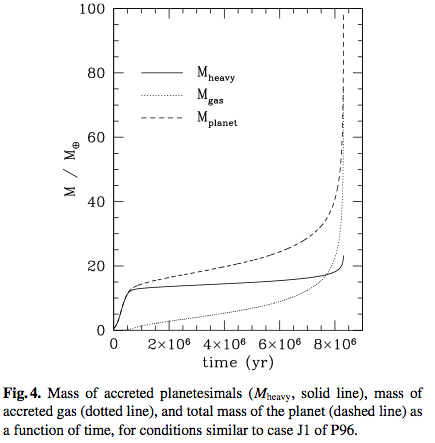
\includegraphics[trim={0cm 2cm 0 0},clip, keepaspectratio,width=0.48\textwidth]{massenvvscore}
\caption{Massa planetaria in funzione della massa del core. Da \cite{alibert2005models}.}\label{fig:massenvvscore}
\end{wrapfigure}

Se il protopianeta raggiunge un valore critico di massa, dipendente debolmente da luminosit\'a generata da accrescimento dei pianetesimi e opacit\'a, per mantenere equilibrio idrostatico l'inviluppo gassoso del pianeta si contrae su tempi scala di Kelvin-Helmholtz. In questa seconda fase l'accresscimento di massa diviene cos\'i rapido da esaurire il gas disponibile nella regione: curva verticale di figura (\ref{fig:massenvvscore}). L'accrescimento di gas has come limite superiore il flusso di gas dovuto a evoluzione viscosa del disco.

Da modelli numerici risulta
\begin{equation}
M_c^{crit}=10\mearth{}(\frac{\dot{M}_c}{\num{e-7}\mearth{}\si{\per\year}})\expy{q}(\frac{\kappa}{\SI{0.1}{\square\meter\per\kilo\gram}})\expy{s}
\end{equation}
con $q,s\approx0.2-0.3$ (\cite{ikoma2000formation}).

\vspace{2cm}

\section{Accrescimento limitato da velocit\'a di raffreddamento}

Seguendo (\cite{mordasini2012characterization}) la struttura del pianeta \'e determinata integrando le equazioni di conservazione di massa, momento e l'equazione del trasporto di energia:
\begin{align}
&\TDy{r}{m}=4\pi r^2\rho\\
%&\TDy{r}{l}=0\\
&\TDy{r}{P}=-\frac{Gm}{r^2}\rho\\
&\TDy{r}{T}=\frac{T}{P}\TDy{r}{P}\nabla(T,P)\\
&\nabla(T,P)=\TDly{P}{T}=\min{(\nad{},\nrad{})}
\end{align}
dove $\nrad{}$ e $\nad{}$ indicano il gradiente radiativo e adiabatico.

La luminosit\'a del pianeta \'e determinata tramite
\begin{equation}
E_t=E_g+E_i=\int_0^M\frac{Gm}{r}\,dm+\int_{M_z}^Mu\,dm=-\xi\frac{GM^2}{2R}
\end{equation}
che sostituita nell'equazione di conservazione dell'energia da:
\begin{equation}
-\TDof{t}E_t=L=L_M+L_R+L_{\xi}=\xi\frac{GM}{R}\dot{M}-\xi\frac{GM^2}{2R^2}\dot{R}+\frac{GM^2}{2R}\dot{\xi}
\end{equation}
con $\dot{M}=\dot{M}_Z+\dot{M}_{XY}$.

Ho indicato la massa di gas legata al core con
\begin{equation}
M_{XY}=4\pi\int_{R_c}^R\rho(r')r'^2\,dr'
\end{equation}
con $R_C$ \'e il raggio del core.

Condizioni al bordo:
\begin{align}
&R=\frac{R_B}{1+R_B/(k_lR_H )},\ P=P_{neb}\\
&\tau=\max{(\rho_{neb}\kappa_{neb}R),2/3)},\ T_i^4=\frac{3\tau L_{int}}{8\pi\sigma R^2}\\
&T^4=T_{neb}^4+T_{int}^4,\ L(R)=L_{int}
\end{align}
$k_{liss}=3-4$, quindi $R_p\approx \min{(R_B,k_{liss}R_H)}$ e introduco il raggio di Bondi
\begin{equation}
R_B=G\frac{M_c}{c_0^2}\approx\SI{4e10}{\cm}a(AU)\expy{1/2}\frac{M_c}{\mearth{}}
\end{equation}
definito come raggio in cui energia termica e potenziale gravitazionale si equivalgono.%il core perturba la pressione del gas del disco.

\begin{workout}[envelope mass as function of core mass]
Armitage 17 eq 232 (`'lecture nite on formation and early evolution of PS)
\begin{equation}
M_{env}\approx\int_{R_c}^{R_o}4\pi r^2\rho\,dr\propto\frac{\sigma}{\kappa_RL}(\frac{\mu m_pGM_t}{4k_b})^4\ln{\frac{R_o}{R_c}}
\end{equation}
\end{workout}

\begin{workout}[Rfes per espressione raggio bondi]

\end{workout}


\begin{workout}[Hydrostatic equilibrium hypothesis]
Characterization of exoplanets from their formation I (eq 10)
\end{workout}


\begin{workout}[Rfes espressione accrescimento gas]
Rate di accrescimento limitato dalla velocit\'a di raffreddamento:
\begin{equation}
\dot{M}_{XY}\propto\ \frac{M_p}{M_*}<(H_P/R_p)^3/\sqrt{3}
\end{equation}
quindi la massa di gas aumenta esponenzialmente a partire da $M_c\approx10\mearth{}$.
\end{workout}

\section{Accrescimento limitato dalla disponibilit\'a di gas del disco}

Se $H\approx R$ il pianeta perturba in maniera non trascurabile il disco (il rate di accrescimento di gas \'e maggiore di quello fornito dal disco). Il raggio del pianeta \'e determinato dalle condizioni al bordo per materia accresciuta tramite free-fall da $R_H$ a $R$:
\begin{align}
&\dot{M}_{XY}=\dot{M}_{XY,max},\ v_{ff}^2=2GM(\frac{1}{R}-\frac{1}{R_H})\\
&P=P_{neb}+\frac{\dot{M}_{XY}}{4\pi r^2}v_{ff}+\frac{2g}{3\kappa},\ \tau=\max{(\rho_{neb}\kappa_{neb}R,2/3)}\\
&T_{int}^4=\frac{3\tau L_{int}}{8\pi\sigma R^2},\ T^4=(1-A)T_{neb}^4+T_{int}^4
\end{align}

In questa fase la velocit\'a di accrescimento di gas \'e determinata dall'evoluzione viscosa del disco:
\begin{equation}
\dot{M}_{e,visc}=f_{hyd}3\pi\nu\Sigma_g
\end{equation}
$f_{hyd}\approx0.9$ valore determinato da simulazioni idrodinamiche (\cite{lubow1999disk}).

\begin{workout}[Bondi accretion rate]
Unperturbed viscous flow
\begin{equation}
\dot{M}_{e,B}\approx\frac{\Sigma_g}{H}(\frac{R_H}{3})^3\Omega
\end{equation}
\end{workout}

\begin{workout}[Detached phase accretion rate]
Characterization of exoplanets from their formation pg 8
\end{workout}

\begin{workout}[Wien displacement]
$\lambda_{max}T\approx \SI{3e-3}{\meter\kelvin}$
\end{workout}

\begin{workout}[Critical core mass]
From toward deterministic
\begin{equation}
M_{c,crit}\approx10(\frac{\dot{M}_c}{\num{e-6}\mearth{}\si{\per\year}})\expy{0.2-0.3}(\frac{\kappa}{\SI{1}{\square\cm\per\gram}})\expy{0.2-0.3}\mearth{}
\end{equation}•
\end{workout}

\begin{workout}[gas accretion refs]
Lissauer 09: Models of Jupiter’s growth incorporating thermal and hydrodynamic constraints
Rafikov 10: ''Constraint on giant planet production by core accretion''
Rafikov 04 Atmospheres of protoplanetary cores: critical mass for nucleated instability.
Refs: Planet formation models: the interplay with the planetesimal disc (Fortier 2013), Characterization of exoplanets from their formation I. Models of combined planet formation and evolution (Mordasini 12)
\end{workout}

\begin{workout}[Planet-Disk exchange in hydrodynamic manner]
Ormel 15/ Cimerman 17
\end{workout}

%\section{Fase isolata}

\begin{workout}[Fase isolata: fonti energia]
fonti energia: tidal heating radiogeninc heat, star flux
\end{workout}


{\let\clearpage\relax\let\cleardoublepage\relax
\chapter{Evoluzione orbite proto-pianeti: migrazione planetaria.}
}

\begin{wrapfigure}[10]{l}{0.5\textwidth}
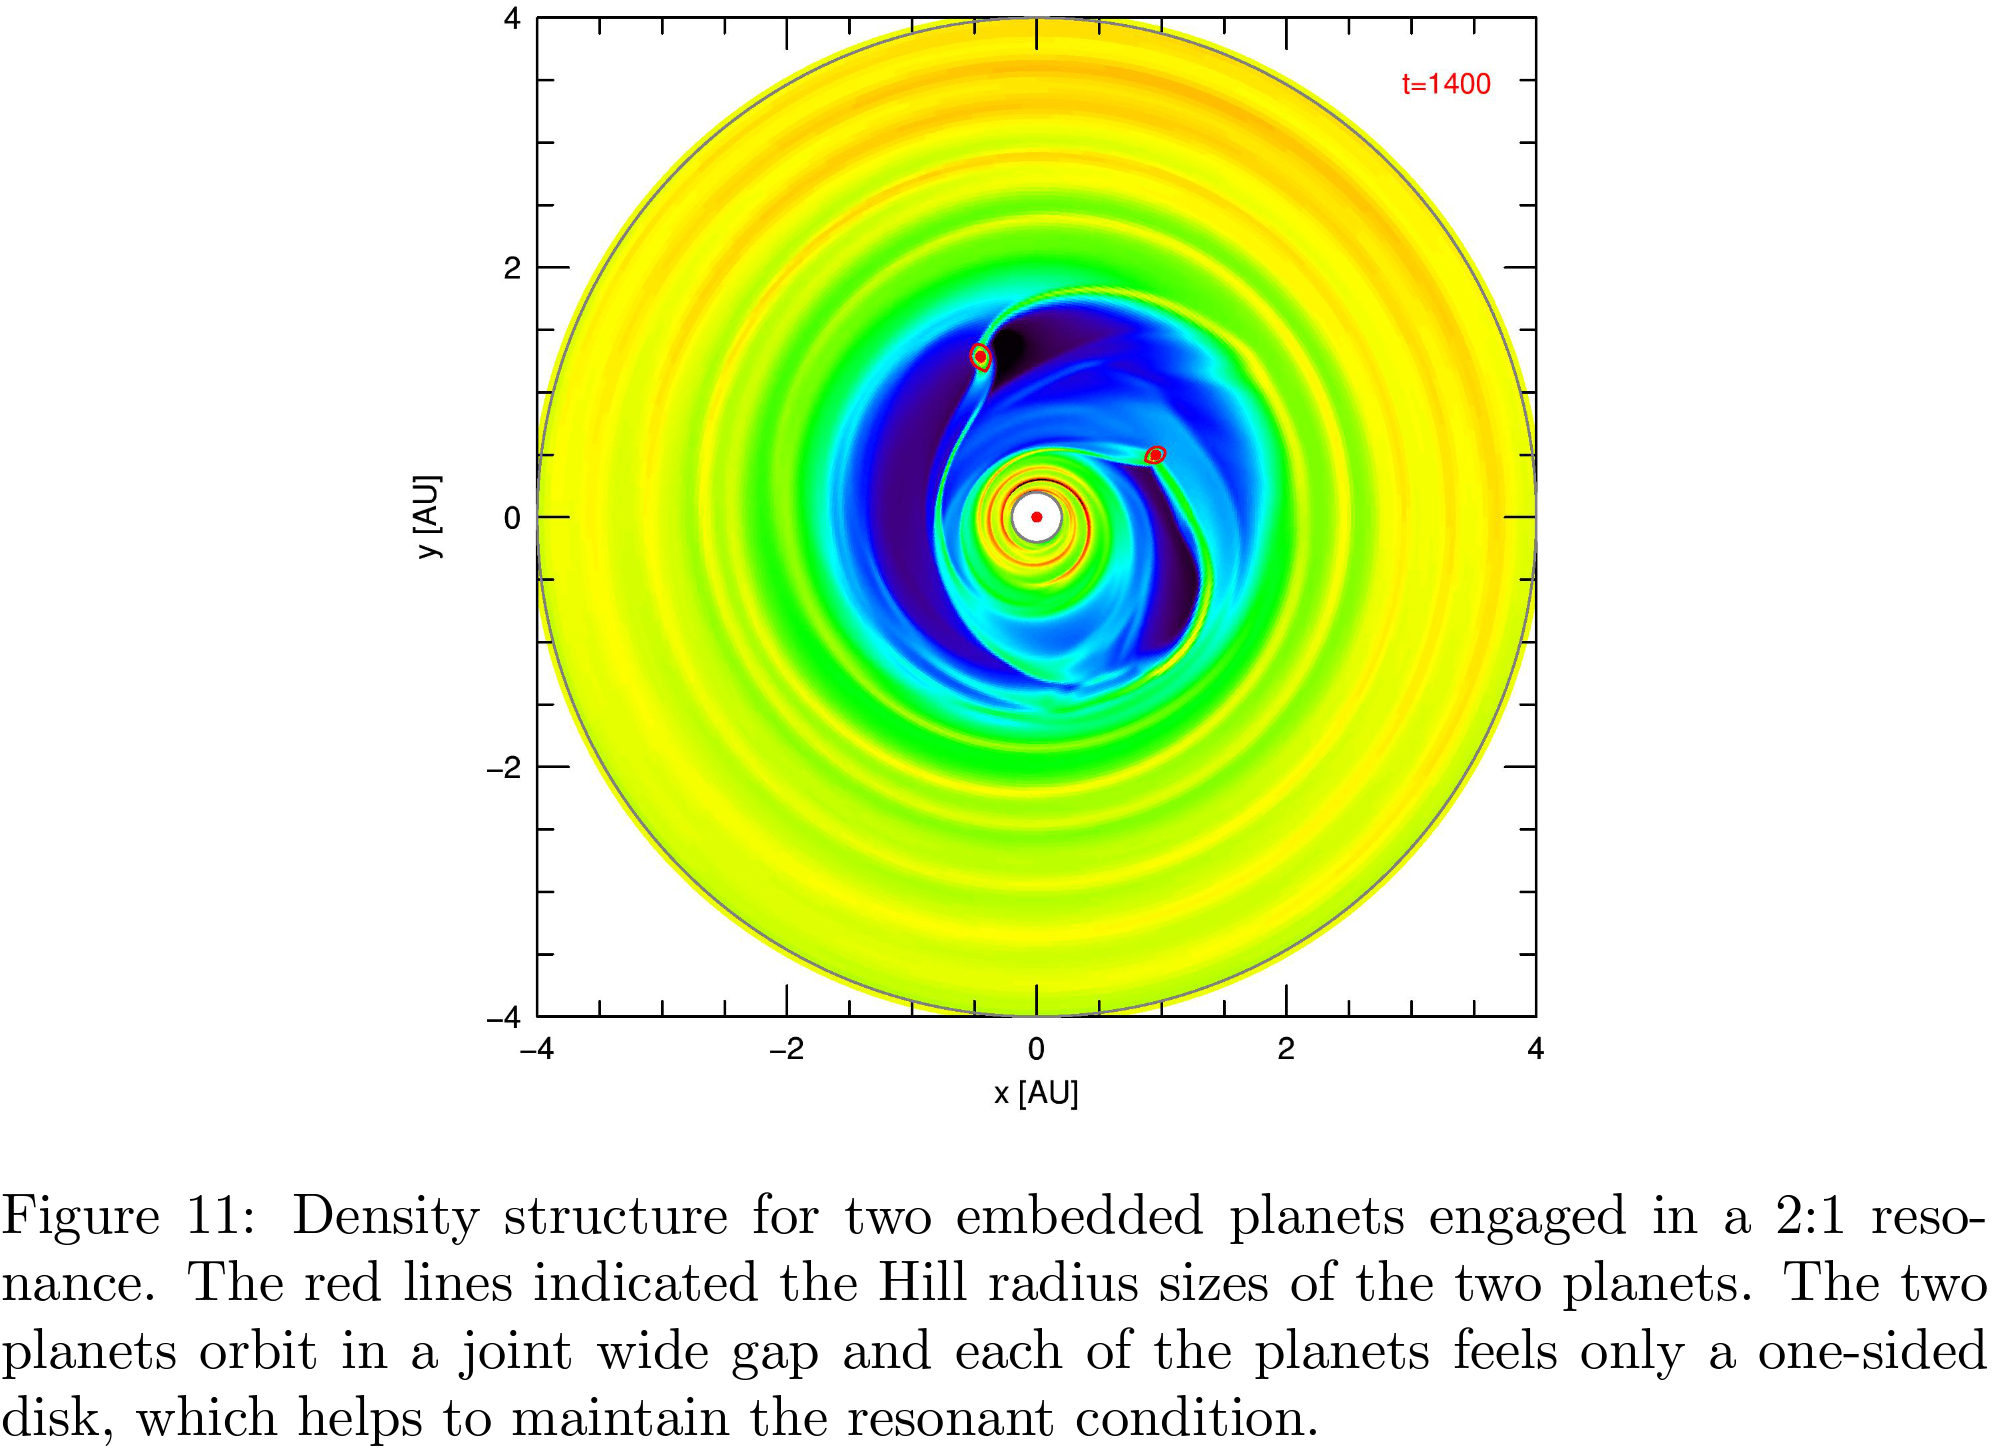
\includegraphics[trim={0cm 11cm 0 0},clip, keepaspectratio,width=0.48\textwidth]{pdres}
\caption{Simulazione evoluzione orbite planetarie in disco di accrescimento fino a cattura in risonanza $2:1$: le regioni pi\'u dense sono in rosso. Da \cite{kley2012planet}.}\label{fig:pdres}
\end{wrapfigure}

L'osservazione di una sottopopolazione di esopianeti giganti su orbite strette, per cui sembra improbabile una formazione in loco, e la presenza di sistemi multipli in risonanza sono indicatori di evoluzione orbitale, d'altra parte nel Sistema solare fenomeni di migrazione fornisco una spiegazione all'orbita di plutone, alla presenza di numerosi oggetti della fascia di Kuiper in risonanza $3:2$ con Nettuno e al periodo di collisioni intense testimoniato da craterizzazione (Late heavy bombardment).

\vspace{1.5cm}

Fenomeni che possono dar luogo a migrazione planetaria:
\begin{itemize}
\item Interazione con disco proto-planetario. Considerando le perturbazioni lineari nella densit\'a del disco prodotte dal potenziale del pianeta si determina la risultante dei momenti torcenti $\Gamma$ dovuti alle risonanze di Lindblad e alla regione di corotazione. Velocit\'a edirezione della migrazione dipendono dalle caratteristiche del disco, massa del pianeta e moto relativo pianeta-gas.


\begin{errata}[Elenco schematicamente alcuni risultati da \cite{armitage2007lecture} e \cite{crida2006planetary}]
 La migrazione di tipo I ha tempi caratteristici
\begin{equation}
\tau_I\propto\frac{M_p}{\Gamma}\propto M_p\expy{-1}
\end{equation}
per pianeta $5\mearth{}$ a \SI{5}{\astronomicalunit} si ha $\tau_I=\SI{0.5}{\mega\year}$.

La migrazione di tipo II \'e caratterizzata da formazione di un gap attorno all'orbita del pianeta: la transizione tra migrazione I e II avviene se $R_H>H$ e momento torcente dovuto alla viscosit\'a del disco \'e minore del momento esercitato dal pianeta sul disco. La velocit\'a di migrazione di tipo II \'e determinata dall'evoluzione viscosa del disco:
\begin{equation}
\dot{a}_p=-\frac{3}{2}\frac{\nu}{r}
\end{equation}
Il momento esercitato sul pianeta dalla regione di corotazione pu\'o dar luogo a feedback positivo su pianeta di massa intermedia con velocit\'a radiale $\dot{a}_p$.
\end{errata}

\item Interazione con disco residuo di planetesimi

\item Interazione tra due o pi\'u pianeti giganti

\item Interazione con stella in sistema di stelle binarie

\item Interazione mareale con la stella

\end{itemize}

%{\let\clearpage\relax\let\cleardoublepage\relax
%\chapter{N-body interactions inside proto disk}
%}


\begin{workout}[Long-term evolution: laplace equations]
The HARPS search for southern extra-solar planets-XXVIII. Up to seven planets orbiting HD 10180: probing the architecture of low-mass planetary systems
\end{workout}
